\section{Performance Study and Testing}

\subsection{Benchmark Setup}

Three scenarios are benchmarked,
each time averaged over 10 runs.
Both wall-clock time (\texttt{timespec\_get}) and CPU time (\texttt{clock()}) are measured.
File sizes tested: 1\,MB, 2\,MB.
File counts: 100, 200, 400, 600, 800, 1000.

\subsection{Analysis}

\begin{table}[h]
\centering
\caption{1\,MB files}
\resizebox{\textwidth}{!}{
\begin{tabular}{lllllllllllll}
\toprule
 & \multicolumn{2}{c}{\textbf{100}} & \multicolumn{2}{c}{\textbf{200}} & \multicolumn{2}{c}{\textbf{400}} & \multicolumn{2}{c}{\textbf{600}} & \multicolumn{2}{c}{\textbf{800}} & \multicolumn{2}{c}{\textbf{1000}} \\
\textbf{Scenario} & wall & cpu & wall & cpu & wall & cpu & wall & cpu & wall & cpu & wall & cpu \\
\midrule
Different sizes      & 0.012 & 0.011 & 0.024 & 0.022 & 0.049 & 0.047 & 0.071 & 0.072 & 0.095 & 0.087 & 0.118 & 0.106 \\
Unique content       & 0.096 & 0.080 & 0.189 & 0.183 & 0.383 & 0.356 & 0.573 & 0.573 & 0.769 & 0.770 & 0.978 & 0.975 \\
Identical content    & 0.143 & 0.144 & 0.286 & 0.286 & 0.580 & 0.580 & 0.859 & 0.833 & 1.143 & 1.097 & 1.435 & 1.428 \\
\bottomrule
\end{tabular}}
\end{table}

\begin{table}[h]
\centering
\caption{2\,MB files}
\resizebox{\textwidth}{!}{
\begin{tabular}{lllllllllllll}
\toprule
 & \multicolumn{2}{c}{\textbf{100}} & \multicolumn{2}{c}{\textbf{200}} & \multicolumn{2}{c}{\textbf{400}} & \multicolumn{2}{c}{\textbf{600}} & \multicolumn{2}{c}{\textbf{800}} & \multicolumn{2}{c}{\textbf{1000}} \\
\textbf{Scenario} & wall & cpu & wall & cpu & wall & cpu & wall & cpu & wall & cpu & wall & cpu \\
\midrule
Different sizes      & 0.012 & 0.011 & 0.023 & 0.023 & 0.047 & 0.047 & 0.070 & 0.070 & 0.095 & 0.095 & 0.118 & 0.119 \\
Unique content       & 0.170 & 0.170 & 0.344 & 0.344 & 0.702 & 0.700 & 1.069 & 1.026 & 1.428 & 1.405 & 1.811 & 1.798 \\
Identical content    & 0.250 & 0.248 & 0.503 & 0.503 & 1.023 & 1.006 & 1.520 & 1.506 & 2.062 & 2.062 & 2.555 & 2.525 \\
\bottomrule
\end{tabular}}
\end{table}

\begin{figure}[h]
\centering
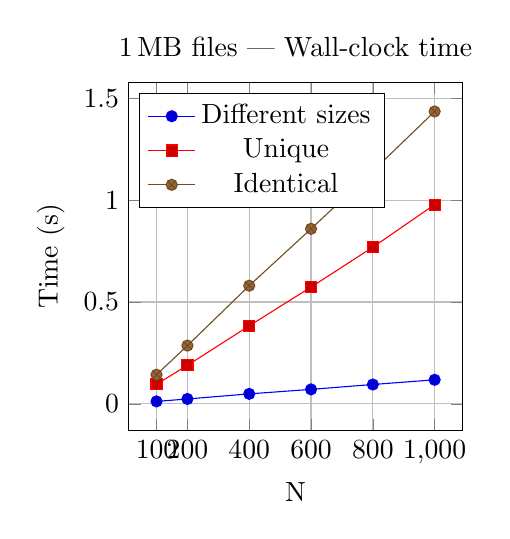
\begin{tikzpicture}
\begin{axis}[
    title={1\,MB files --- Wall-clock time},
    xlabel={N},
    ylabel={Time (s)},
    legend pos=north west,
    grid=major,
    width=0.48\textwidth,
    height=6cm,
    xtick={100,200,400,600,800,1000},
]
\addplot coordinates {(100,0.012) (200,0.024) (400,0.049) (600,0.071) (800,0.095) (1000,0.118)};
\addplot coordinates {(100,0.096) (200,0.189) (400,0.383) (600,0.573) (800,0.769) (1000,0.978)};
\addplot coordinates {(100,0.143) (200,0.286) (400,0.580) (600,0.859) (800,1.143) (1000,1.435)};
\legend{Different sizes, Unique, Identical}
\end{axis}
\end{tikzpicture}
\hfill
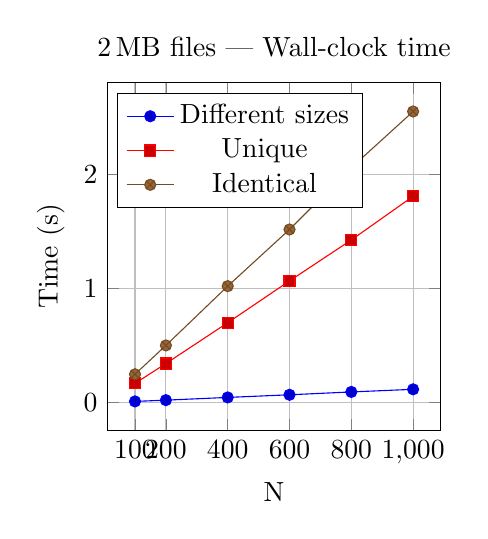
\begin{tikzpicture}
\begin{axis}[
    title={2\,MB files --- Wall-clock time},
    xlabel={N},
    ylabel={Time (s)},
    legend pos=north west,
    grid=major,
    width=0.48\textwidth,
    height=6cm,
    xtick={100,200,400,600,800,1000},
]
\addplot coordinates {(100,0.012) (200,0.023) (400,0.047) (600,0.070) (800,0.095) (1000,0.118)};
\addplot coordinates {(100,0.170) (200,0.344) (400,0.702) (600,1.069) (800,1.428) (1000,1.811)};
\addplot coordinates {(100,0.250) (200,0.503) (400,1.023) (600,1.520) (800,2.062) (1000,2.555)};
\legend{Different sizes, Unique, Identical}
\end{axis}
\end{tikzpicture}
\caption{Wall-clock time vs number of files}
\end{figure}

\begin{figure}[h]
\centering
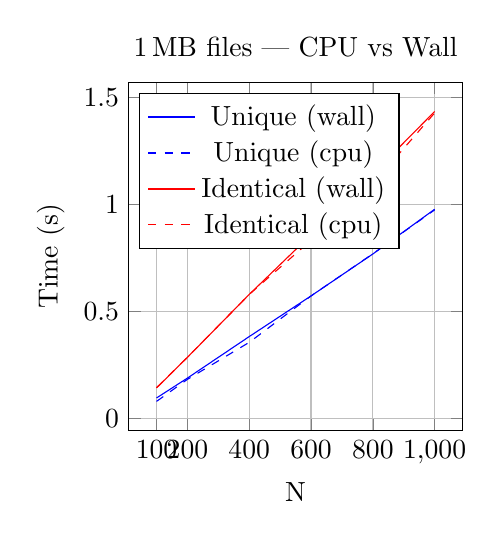
\begin{tikzpicture}
\begin{axis}[
    title={1\,MB files --- CPU vs Wall},
    xlabel={N},
    ylabel={Time (s)},
    legend pos=north west,
    grid=major,
    width=0.48\textwidth,
    height=6cm,
    xtick={100,200,400,600,800,1000},
]
\addplot[blue, solid] coordinates {(100,0.096) (200,0.189) (400,0.383) (600,0.573) (800,0.769) (1000,0.978)};
\addplot[blue, dashed] coordinates {(100,0.080) (200,0.183) (400,0.356) (600,0.573) (800,0.770) (1000,0.975)};
\addplot[red, solid] coordinates {(100,0.143) (200,0.286) (400,0.580) (600,0.859) (800,1.143) (1000,1.435)};
\addplot[red, dashed] coordinates {(100,0.144) (200,0.286) (400,0.580) (600,0.833) (800,1.097) (1000,1.428)};
\legend{Unique (wall), Unique (cpu), Identical (wall), Identical (cpu)}
\end{axis}
\end{tikzpicture}
\hfill
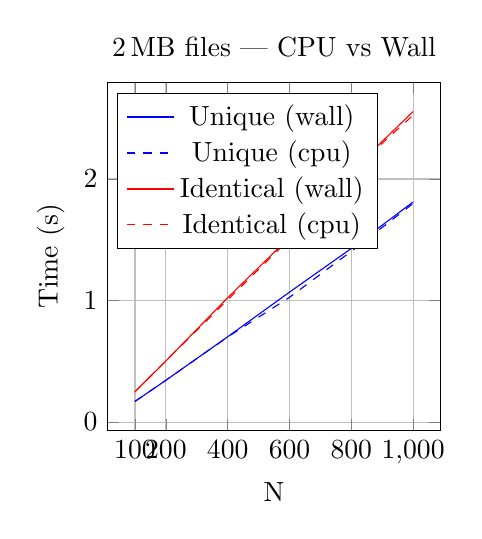
\begin{tikzpicture}
\begin{axis}[
    title={2\,MB files --- CPU vs Wall},
    xlabel={N},
    ylabel={Time (s)},
    legend pos=north west,
    grid=major,
    width=0.48\textwidth,
    height=6cm,
    xtick={100,200,400,600,800,1000},
]
\addplot[blue, solid] coordinates {(100,0.170) (200,0.344) (400,0.702) (600,1.069) (800,1.428) (1000,1.811)};
\addplot[blue, dashed] coordinates {(100,0.170) (200,0.344) (400,0.700) (600,1.026) (800,1.405) (1000,1.798)};
\addplot[red, solid] coordinates {(100,0.250) (200,0.503) (400,1.023) (600,1.520) (800,2.062) (1000,2.555)};
\addplot[red, dashed] coordinates {(100,0.248) (200,0.503) (400,1.006) (600,1.506) (800,2.062) (1000,2.525)};
\legend{Unique (wall), Unique (cpu), Identical (wall), Identical (cpu)}
\end{axis}
\end{tikzpicture}
\caption{CPU time vs Wall-clock time comparison}
\end{figure}

\textbf{Linear scaling in N.}
All scenarios show linear growth.
For unique files at 1\,MB: 0.096\,s at N=100 scales to 0.978\,s at N=1000
(9.8$\times$ increase from a 10$\times$ increase in N), confirming $O(N)$ total complexity.

\textbf{Different sizes is constant per file.}
The different sizes row is nearly independent of file size
(0.118\,s for both 1\,MB and 2\,MB at N=1000), because file content is
never read---only \texttt{file\_size} is called.

\textbf{Linear scaling in S.}
Comparing unique content at N=1000: 0.978\,s for 1\,MB vs 1.811\,s for 2\,MB---a
factor of $\approx$1.85$\times$, close to the expected 2$\times$ for a 2$\times$
increase in file size.
This confirms $O(S)$ per-file cost when content hashing is required.

\textbf{Identical files are slower than unique.}
Duplicates require both hashing and byte-by-byte comparison to confirm
identity.
At N=1000 with 1\,MB files, identical content takes 1.435\,s vs 0.978\,s
for unique---a factor of $\approx$1.47$\times$, consistent with the additional
file reads needed for equality verification.

\subsection{Testing}

Unit tests were written for three modules: \textbf{Vector}, \textbf{Hashmap} and \textbf{FILEDEDUP}.
